
\FloatBarrier
\section{Система Рёсслера} %  % {{{1 _ROSS_
\label{atu:sect:ross}

\LinkRef{
  ross: ASAU-14. ISDMCI-2011, ISDMCI-2012
  % ~/doc/tex/asau/asau14/atu/atu.tex
}

\subsection{Определение системы и анализ её динамики} %  % {{{2 _ross_task

In~\cite{neimark_stoch_chaos_vibro,koltsova_nl_dyn_chem,berje_order_in_chaos,chulichkcov_mm_ml_dyn}

\begin{equation}
\begin{cases}
  \dot{x}  = -y - z  ,  \\
  \dot{y}  = x + a y ,\\
  \dot{z}  = b + z \cdot ( x-c ) .
\end{cases}
\label{atu:eq:rossler}
\end{equation}

Здесь \(x\), \(y\), \(z\) -- переменные состояния системы,
которые соответствуют концентрациям основных реагентов
в моделируемой химической системе.
Соответственно \(a\), \(b\), \(c\) --
параметры, определяющие динамику системы
(в моделируемой системе определяются константами химического равновесия
и концентрациями вспомогательных реагентов).

При моделировании данной системы положим
\(a=0.25\), \(b=1\).
В этом случае параметр \(c\) определяет
тип динамики системы.
Определение значения данного параметра и будет
целью задачи идентификации.

В данной системе нет внешнего входного сигнала \( u(t) \).
Это объясняется тем, что за счет 
поддержания постоянных концентраций вспомогательных
компонент, постоянного пополнения исходных веществ
и удаления продуктов реакции система обладает
собственным источником энергии, который обеспечивает
динамику системы и при отсутствии 
внешнего воздействия.

Как и другие системы хаотической динамики, система Ресслера
не позволяет построить систему идентификации, основанную
на формировании критерия качества идентификации
как меры близости непосредственных значений выходных сигналов
объекта \( x_0(t) \) и модели \( x_m(t) \).
Более того, сам вид поведения данной системы может значительно изменяться
при малых изменениях параметров, совершая переход от
хаотического к сложно-периодическому и обратно.

При малых значениях параметра (\(c \approx 2 \))
система проявляет регулярную динамику,
совершая колебательное движение вокруг точки неустойчивого равновесия.
При увеличении значения параметра \(c\) происходит удвоение периода,
поведение системы становится все более сложным, и в определенном
диапазоне значений параметра система демонстрирует хаотическую динамику.

Идентифицируемый параметр:
$ c \in [2; 50] $, $c_0=5.88$.

Остальные параметры:
\( a \in (0, 0.35 ) \), $a_0=0.25$,
\(b \in[0;4] \), $b_0=1$.

\begin{figure}[htb!]
\centerline{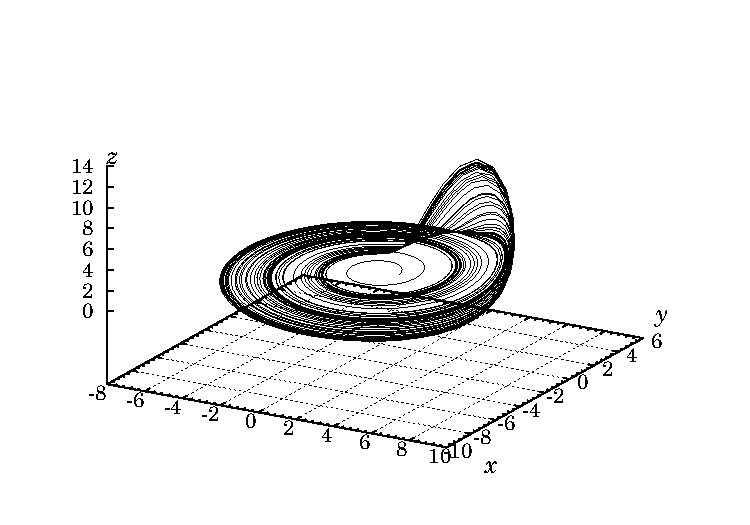
\includegraphics[width=0.6\textwidth]{p/cha/ross_phase3.pdf} }
\caption{Аттрактор системы Рёсслера (\ref{atu:eq:rossler})}
\label{atu:f:ross_phase}
\end{figure}

% }}}2

\subsection{Анализ и выбор критериев}  % {{{2

Критерий
$ z_{\max}$, $ \overline{z} $.

% }}}2

\subsection{Тестовая задача идентификации для системы Рёсслера}  % {{{2


% }}}2

\subsection{Влияние параметров системы идентификации на ошибку идентификации для системы Рёсслера}  % {{{2

% }}}2

\subsection{Зависимости значений критериев идентификации при изменении двух параметров системы Рёсслера}  % {{{2

% }}}2



\subsection{Выводы}  % {{{2

Выводы

% }}}2


% }}}1

% vim: fdm=marker ft=tex
